\documentclass[border=10pt]{standalone}
\usepackage[svgnames]{xcolor}
\usepackage{amsmath}
\usepackage{pgfplots}
\pgfplotsset{compat=newest}
\usepackage[sfdefault]{FiraSans}
\usepackage{FiraMono}
\renewcommand*\familydefault{\sfdefault}
\begin{document}
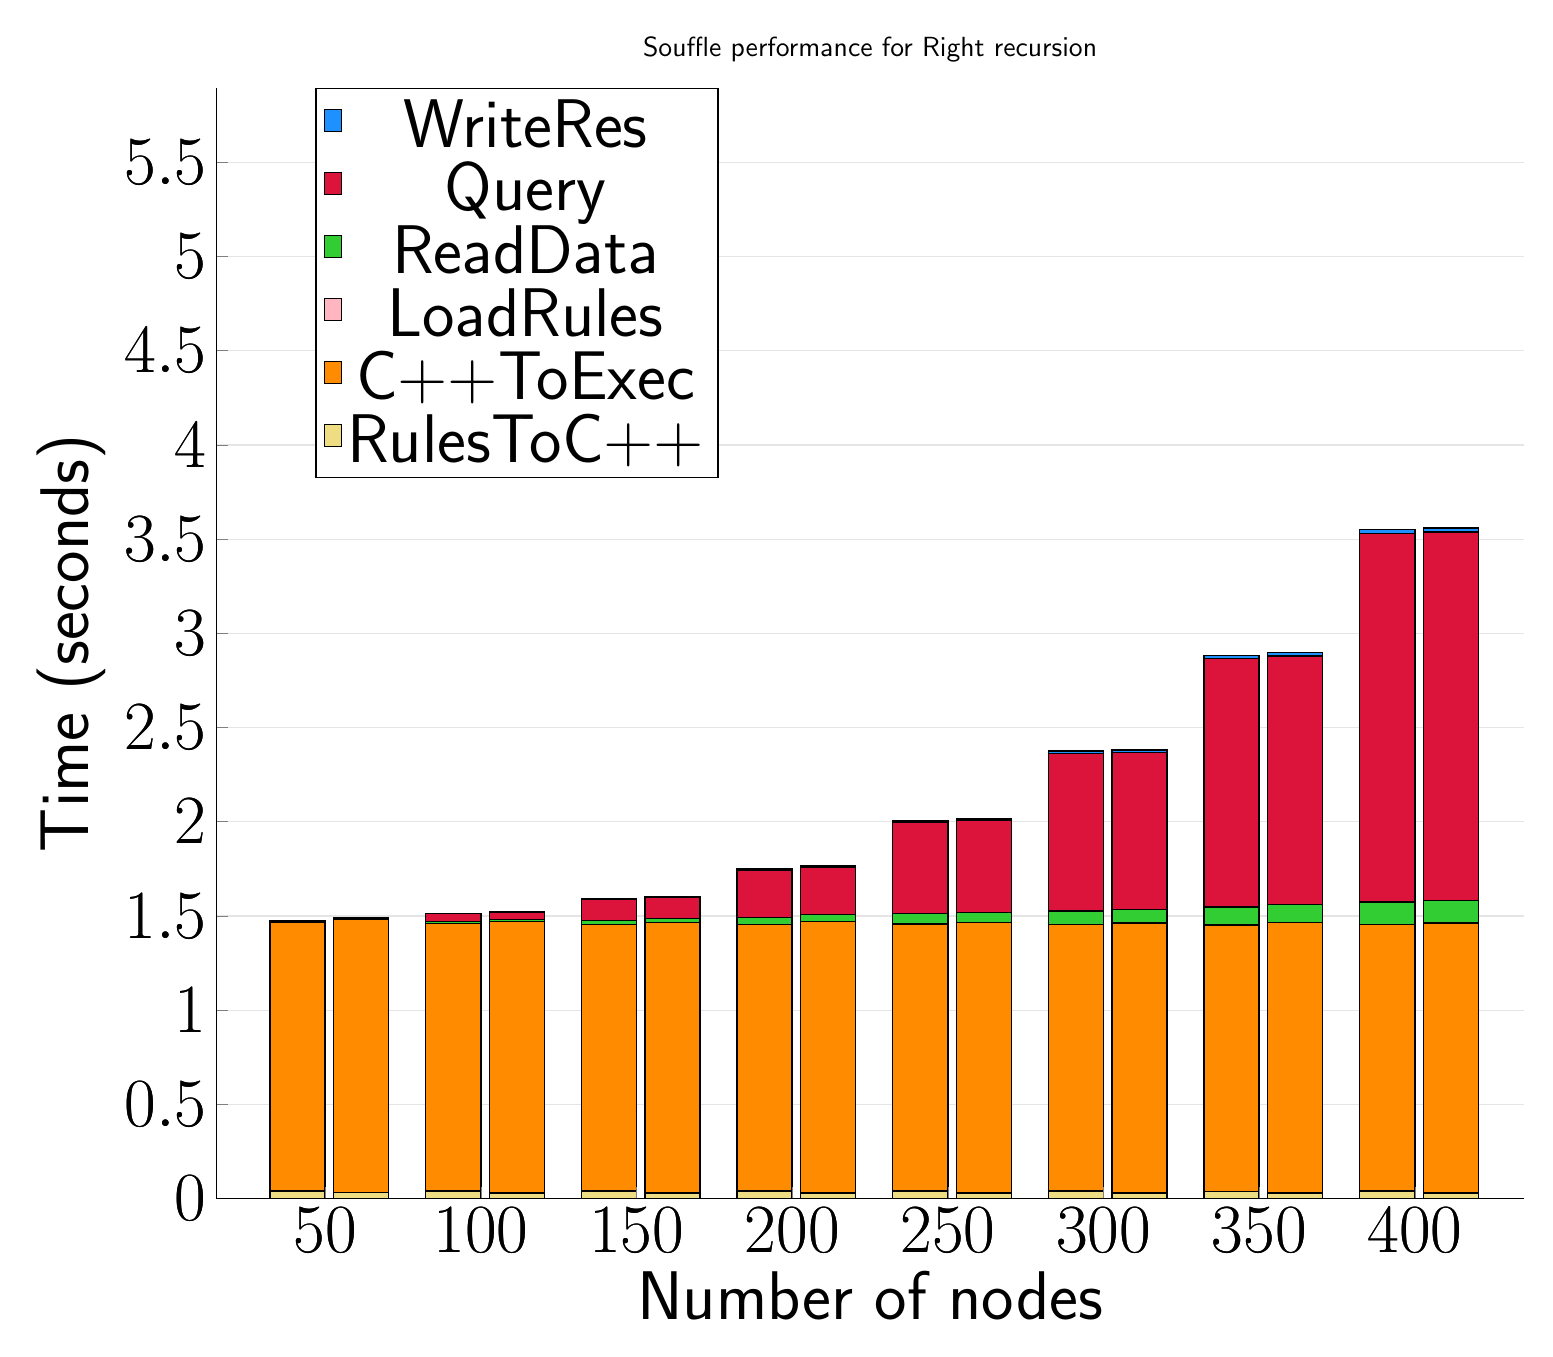
\begin{tikzpicture}
\begin{axis}[
   ybar stacked,
   title={Souffle performance for Right recursion},
   bar shift=-10pt,
   width=1.5\textwidth,
   bar width=0.7cm,
   ymajorgrids, tick align=inside,
   major grid style={draw=gray!20},
   xtick=data,
   ymin=0, ymax=5.895328,
   axis x line*=bottom,
   axis y line*=left,
   enlarge x limits=0.1,
   legend style={
       at={(0.23, 1)},
       anchor=north,
       legend columns=1,
       font=\Huge,
   },
   ylabel={Time (seconds)},
   xlabel={Number of nodes},
   label style={font=\Huge},
   tick label style={font=\Huge},
]
\addlegendimage{fill=DodgerBlue, draw=black, line width=0.2pt}
\addlegendentry{WriteRes}
\addlegendimage{fill=Crimson, draw=black, line width=0.2pt}
\addlegendentry{Query}
\addlegendimage{fill=LimeGreen, draw=black, line width=0.2pt}
\addlegendentry{ReadData}
\addlegendimage{fill=LightPink, draw=black, line width=0.2pt}
\addlegendentry{LoadRules}
\addlegendimage{fill=DarkOrange, draw=black, line width=0.2pt}
\addlegendentry{C++ToExec}
\addlegendimage{fill=LightGoldenrod, draw=black, line width=0.2pt}
\addlegendentry{RulesToC++}
\addplot +[fill=LightGoldenrod, draw=black, line width=0.5pt] coordinates {
    (50, 0.040999984741210936)
    (100, 0.04000000953674317)
    (150, 0.039999961853027344)
    (200, 0.04100000858306885)
    (250, 0.04000003337860107)
    (300, 0.04000000953674317)
    (350, 0.03899998664855957)
    (400, 0.04100000858306885)
};
\addplot +[fill=DarkOrange, draw=black, line width=0.5pt] coordinates {
    (50, 1.4250000238418579)
    (100, 1.4209999799728394)
    (150, 1.4140000581741332)
    (200, 1.4129999876022339)
    (250, 1.4170000076293945)
    (300, 1.415999960899353)
    (350, 1.4119999647140502)
    (400, 1.4130000114440917)
};
\addplot +[fill=LightPink, draw=black, line width=0.5pt] coordinates {
    (50, 1.00667e-05)
    (100, 0.0)
    (150, 2.1883299999999998e-05)
    (200, 2.0395800000000002e-05)
    (250, 0.0)
    (300, 1.04083e-05)
    (350, 0.0)
    (400, 1.04875e-05)
};
\addplot +[fill=LimeGreen, draw=black, line width=0.5pt] coordinates {
    (50, 0.002737379)
    (100, 0.010628269999999999)
    (150, 0.02207617)
    (200, 0.03762241)
    (250, 0.05499152)
    (300, 0.07129216)
    (350, 0.09711057)
    (400, 0.12040999999999999)
};
\addplot +[fill=Crimson, draw=black, line width=0.5pt] coordinates {
    (50, 0.006235963)
    (100, 0.040190109999999994)
    (150, 0.1115031)
    (200, 0.25212199999999996)
    (250, 0.4863906)
    (300, 0.8351862999999999)
    (350, 1.3186430000000002)
    (400, 1.9556050000000003)
};
\addplot +[fill=DodgerBlue, draw=black, line width=0.5pt] coordinates {
    (50, 0.0006429791)
    (100, 0.001710551)
    (150, 0.003699243)
    (200, 0.005976067)
    (250, 0.009188694999999998)
    (300, 0.012767329999999999)
    (350, 0.01726681)
    (400, 0.02236556)
};
\end{axis}
\begin{axis}[
   ybar stacked,
   bar shift=13pt,
   width=1.5\textwidth,
   bar width=0.7cm,
   ymajorgrids, tick align=inside,
   major grid style={draw=none},
   xtick=data,
   ymin=0, ymax=5.895328,
   axis x line*=none,
   axis y line*=none,
   enlarge x limits=0.1,
   label style={font=\Huge},
   tick label style={font=\Huge},
]
\addplot +[fill=LightGoldenrod, draw=black, line width=0.5pt] coordinates {
    (50, 0.033)
    (100, 0.030000000000000006)
    (150, 0.030000000000000006)
    (200, 0.030000000000000006)
    (250, 0.030000000000000006)
    (300, 0.030000000000000006)
    (350, 0.030000000000000006)
    (400, 0.030000000000000006)
};
\addplot +[fill=DarkOrange, draw=black, line width=0.5pt] coordinates {
    (50, 1.448)
    (100, 1.4389999999999998)
    (150, 1.4349999999999998)
    (200, 1.4389999999999996)
    (250, 1.4349999999999998)
    (300, 1.4329999999999998)
    (350, 1.4349999999999996)
    (400, 1.4329999999999998)
};
\addplot +[fill=LightPink, draw=black, line width=0.5pt] coordinates {
    (50, 0.0)
    (100, 0.0)
    (150, 2.16e-05)
    (200, 2.03e-05)
    (250, 0.0)
    (300, 1.0399999999999999e-05)
    (350, 0.0)
    (400, 1.0399999999999999e-05)
};
\addplot +[fill=LimeGreen, draw=black, line width=0.5pt] coordinates {
    (50, 0.0026730000000000005)
    (100, 0.0105891)
    (150, 0.0219944)
    (200, 0.0375268)
    (250, 0.054893199999999996)
    (300, 0.07124079999999999)
    (350, 0.0969935)
    (400, 0.12030420000000001)
};
\addplot +[fill=Crimson, draw=black, line width=0.5pt] coordinates {
    (50, 0.006233)
    (100, 0.040098600000000005)
    (150, 0.1114307)
    (200, 0.2520518)
    (250, 0.4860805)
    (300, 0.8343223999999999)
    (350, 1.3182200000000002)
    (400, 1.954606)
};
\addplot +[fill=DodgerBlue, draw=black, line width=0.5pt] coordinates {
    (50, 0.0006344)
    (100, 0.0015956999999999998)
    (150, 0.0032696999999999995)
    (200, 0.0057109000000000005)
    (250, 0.0088309)
    (300, 0.0125509)
    (350, 0.0170472)
    (400, 0.022152500000000002)
};
\end{axis}
\end{tikzpicture}

\end{document}
